\chapter{Validation of system}
\label{Kap4}

The fourth chapter gives information about several planned tests as well as their test results are discussed in section \ref{tests}.

\section{Planned tests}

\subsection{Test scenario}

The following section describes a test scenario. 
The system is devoted to be used in a context where a nurse has to administer several drugs to many patients in a hospital. With the proposed system, the nurse can control and capture each time she is administering a drug to a patient. The system will check if the selected drug (which was detected in the patient's room) is valid and if it can be administered to the patient. For example, the nurse is walking with a trolley (containing several drugs) on the hallway of a department in the hospital. On the hallway, there are two antennas which are connected to a reader installed nearby. When passing close to antennas, the detected drugs will be automatically stored into the MongoDB database and displayed on the mobile phone or tablet. 
When entering the patient's room, a second antenna detects the drugs and transmits the signal to the reader which receives the information about the location of the drug ('drug X detected in room 314'). After that, if the nurse wants to administer a drug, the system checks whether it was already administered and whether it is permissible. After having administered the selected drug, the event will change to 'already administered in room X' and will be stored in the database. 

\section{Test results}

\subsection{Functional tests}

In order to test the real-time synchonization, all entries in the database were deleted and the application was refreshed (by using the pull-to-refresh plugin). After five seconds, the alert dialog which explains that there are no entries in the database and no detected drugs is displayed (tested 06 June 2018). 

\subsection{Device tests}

The application was tested on four devices including both tablets and smartphones. During development, mainly the iOS simulator was used to rapidly execute and synchronize the application. Since installing a prototype app on an iOS device requires several developer certificates and some configuration steps, it was easier to use the included simulator which is offered by XCode. 
Later, when the app could be executed without throwing any errors, it was installed and tested on an iPhone 7 (Model: 15F79, iOS 11.4). Furthermore, it was installed on an iPad (iOS 11.4) and ran successfully. 
Moreover, the app was tested on two Android devices: a smartphone (Samsung Galaxy S3, Model: GT-9300, Android 4.3) as well as a tablet (Model: Samsung GT-P5110, Android 4.2.2, screen size: 10.1'').
The successful test results can be seen in figure \ref{fig:s3_screenshots}. The figure shows the screenshots of the smartphone "Samsung S3 GT I9300".

\begin{figure}
\centering
\subfigure{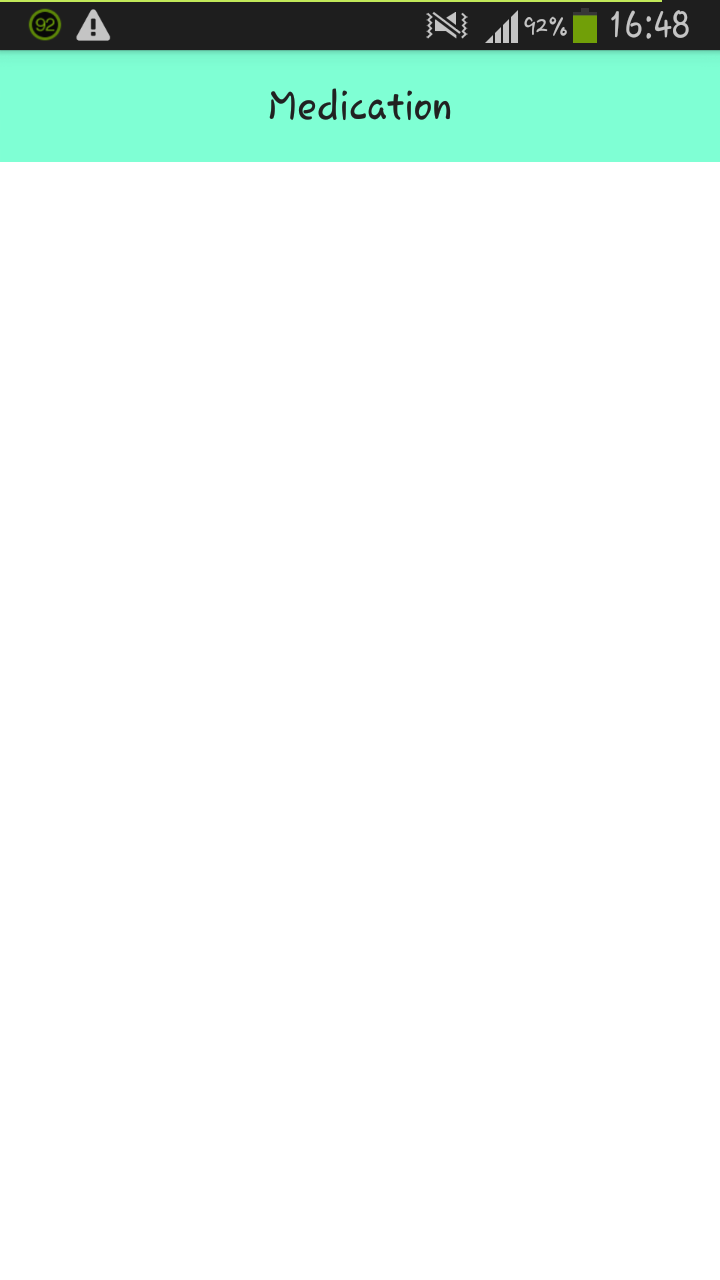
\includegraphics[width=6cm, height=10cm]{s3_01}}
\subfigure{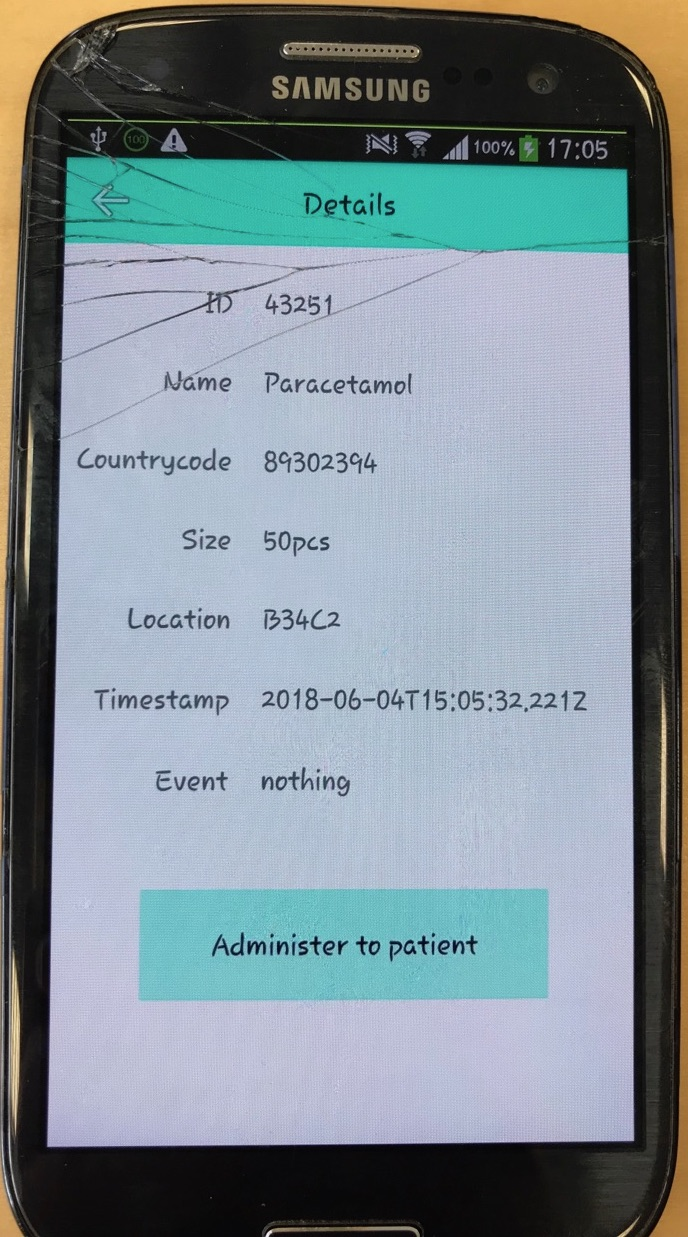
\includegraphics[width=6cm, height=10cm]{s3_02}}
\subfigure{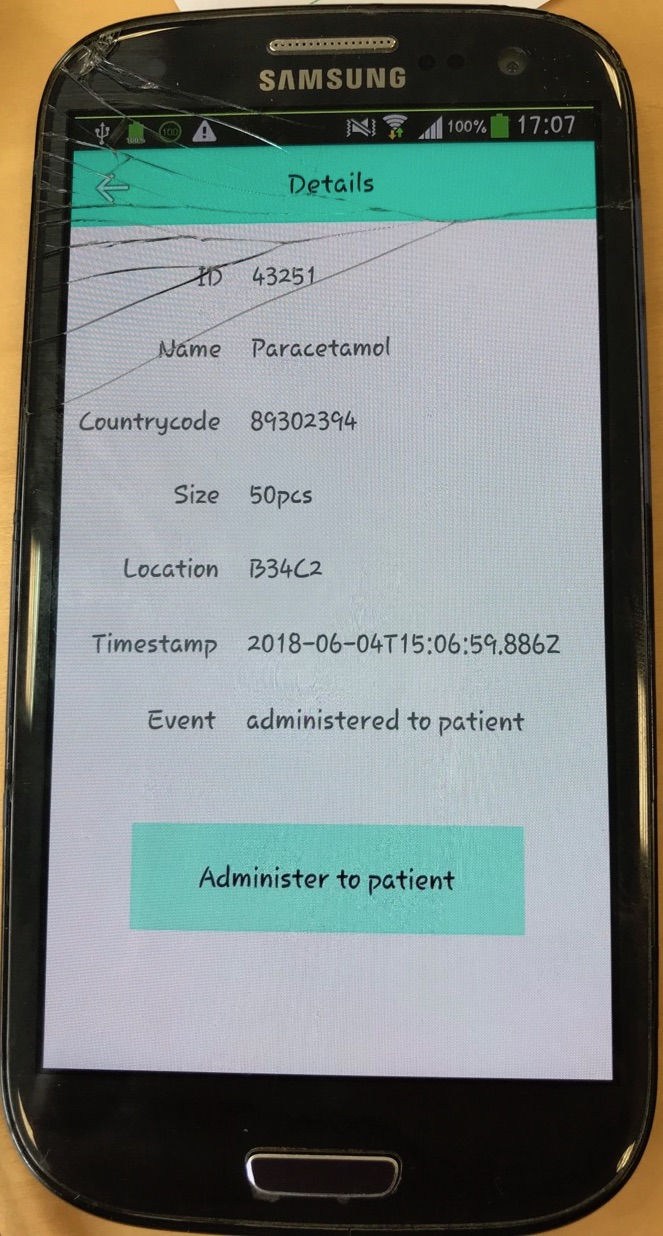
\includegraphics[width=6cm, height=10cm]{s3_03}}
\subfigure{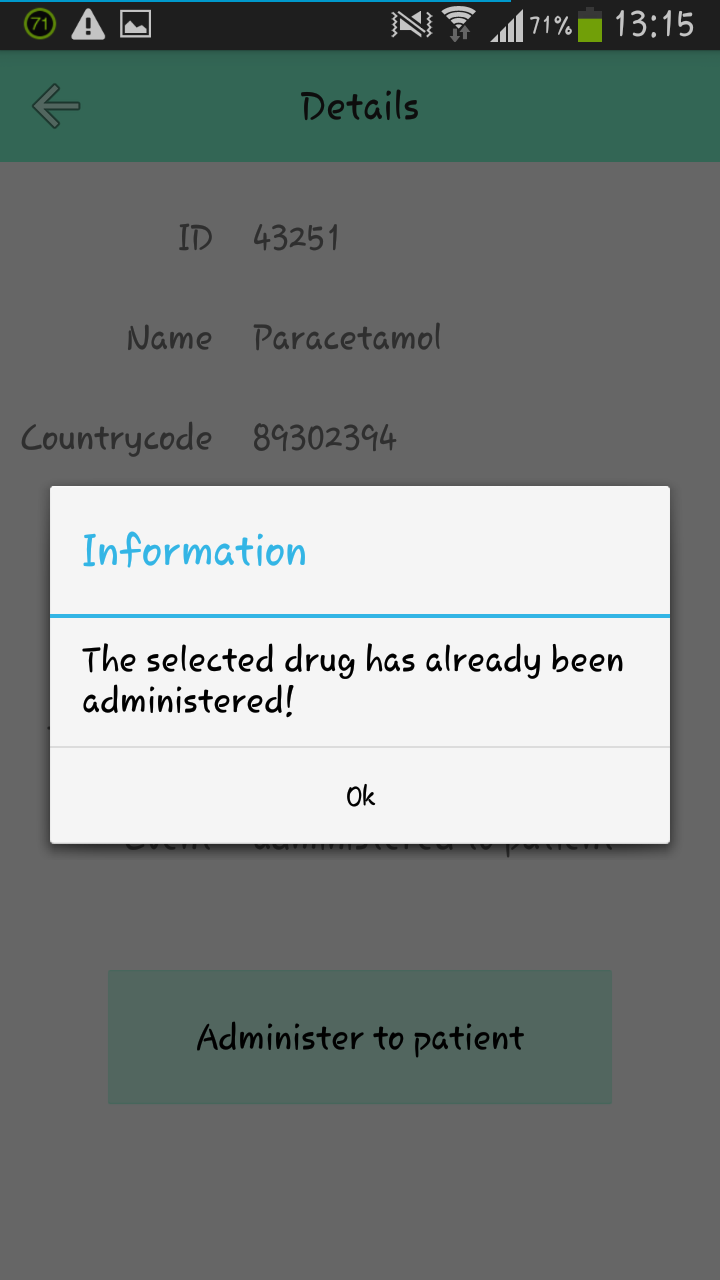
\includegraphics[width=6cm, height=10cm]{s3_04}}
\caption{\label{fig:s3_screenshots} Test screenshots, Samsung S3 GT I9300}
\end{figure}

\subsection{Migration tests}\label{tests}

\ac{HUCA} located in Oviedo, depends on the 'Servicio de Salud del Principado de Asturias' \cite{huca}. Since 28 February 1990, HUCA has been accredited as University Hospital University Hospital due to the cooperation with the university of Oviedo.

HUCA provides 944 beds, 25 operating suites, 238 rooms for external surgical as well as two gamma cameras (\ac{SPECT}/\ac{TC}) \cite{huca}. Altogether, HUCA is divided into 43 medical services, such as alergology, clinical analysis, clinical biochemistry, general surgery, Nephrology, Neurology, Rehabilitation, prevention of work-related risks, radiodiagnostics etc. 

Besides, HUCA forms a part of the 'unit of national reference for work-related illnesses of the respiratory system'. Together with the 'Hospital Monte Naranco', 'hospital del Área Sanitaria IV' and with reference to \ac{SESPA} 'Servicio de Salud del Principado de Asturias' and finally the 'Instituto Nacional de Silicosis', HUCA promotes research on the subject of respiratory disease and its preventions measures.

Figure \ref{fig:permission} shows the permission letter, signed by the director Gloria Herías Corral of HUCA on 8 May 2018 in Oviedo.
Tests were conducted in June 2018.

\begin{figure}
\centering
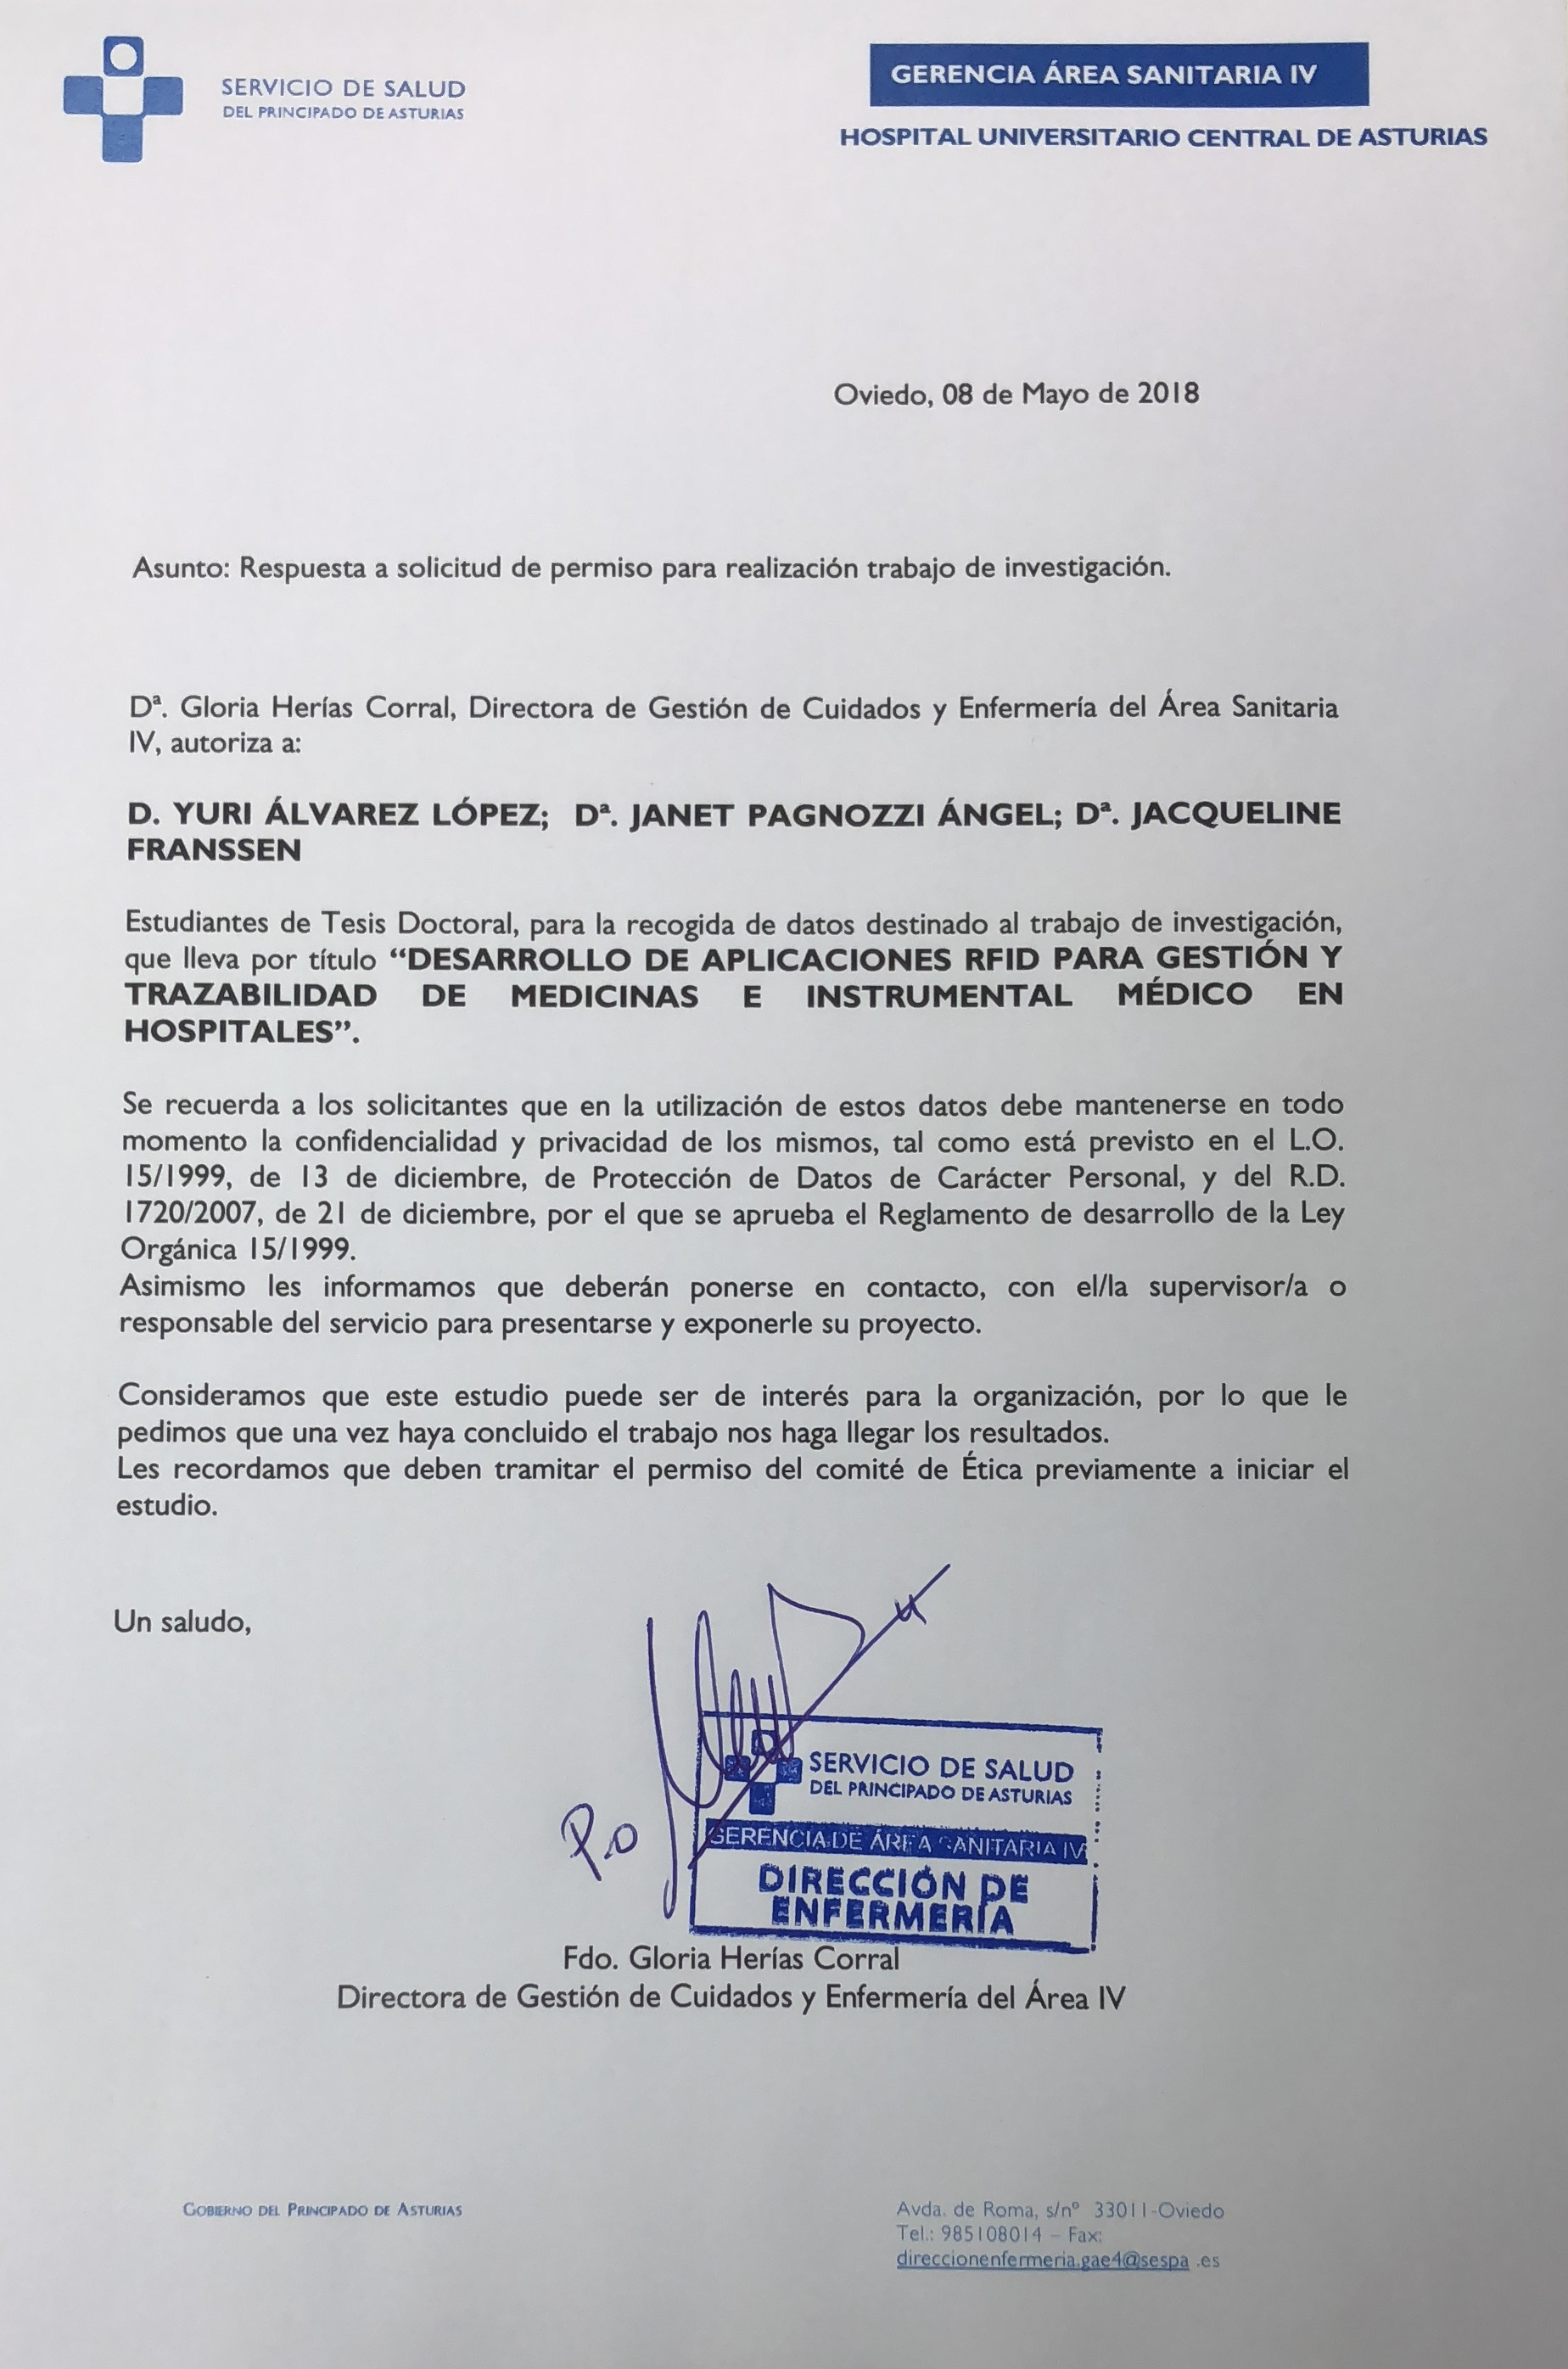
\includegraphics[width=\textwidth]{permission_HUCA} 
\caption{\label{fig:permission}Permission letter about application tests in HUCA} 
\end{figure}

\section{Evaluation of test results}

During the first tests in the HUCA on Monday, on 25/06/2018, some small features of the application were noticed negatively. For instance, the "real-time" synchronization between the mobile device and the database. The reading process of the RFID reader and the following insertion process into the database did work without problems, but the Socket.IO connection between the mobile client and the database server has to be optimized. Moreover, the feature of pulling down the app to refresh all data turned out to be rather obstructive than useful. To solve this problem, a function which automatically reloads the app's main page has to be implemented. These two features have been successfully fixed in the latest version of the application.